\section{Evaluation} 
\label{s:evaluation}
%\fixme{I deleted the subsection Evaluation and change "Outbound Latency" to Evaluation}

In this section, we use large-scale simulations with various topologies and
workloads to study 
%\fixme{change Mazu to the proposed techniques} the proposed techniques'
our techniques' effectiveness in meeting the needs of management
applications that require low-latency control of data plane
state. We consider three applications: failover in a tunneled WAN, 
two-level responsive traffic engineering, and
%\linebreak 
MicroTE~\cite{microte}.
%impact of delays imposed by outbound latencies and the improvements offered
%by Mazu. 
Our simulations leverage switch latency models derived from our measurements
(\secref{s:outbound_meas}).

\subsection{Failover in a Tunneled WAN}%Macro Benchmarks}%Flow Engineering} 
\label{s:fe_eval}

We first evaluate the effectiveness of flow engineering (\FE) and rule offload
(\RO) in the context of a control application that performs failover when a
link fails in  a tunneled WAN.

%To evaluate the effectiveness of Mazu's flow engineering technique, we simulate a failover scenario in a tunneled WAN network, where a random link experiences a failure. 

\minisection{Topology} We use a simple full mesh (overlay) network of 25
nodes.  The tunnels between these nodes share the same physical network. Each
tunnel has between 5 and 10 intermediate switches. Per link capacity lies in
$[100,1000]$.

\minisection{Workloads} We consider six workloads (\tabref{qosTable}). For
each workload,
%\minisection{Traffic matrix} 
we assign a popularity index (random number
within an internal) to each node. The number of flows between a pair
of nodes is proportional to the product of their popularities. Each flow
imposes a unit demand. At the start of our simulation, the traffic is routed
such that the maximum load on any link is minimized.
% . The product of popularity index between any two nodes indicates the
% volume of traffic between them. Initially we map the generate traffic
% matrix to the network

\minisection{Table occupancy} We assume that the new rules being installed
upon failure (some of these could be updates to existing rules) all have the
same priority $P$. Further, we assume that the tunnel end-points already have
some lower priority rules, a subset of which are displaced by the new
rules. We randomly pick the number of such displaced rules within some
interval (defined for each workload in \tabref{qosTable}). For simplicity, we
assume that there are no dependencies across rules; we consider dependencies
in subsequent sections.

\newcommand{\sA}{{\em s1}}
\newcommand{\sB}{{\em s2}}
\newcommand{\sC}{{\em s3}}
\newcommand{\sD}{{\em s4}}
\newcommand{\sE}{{\em s5}}
\newcommand{\sF}{{\em s6}}

\begin{table}
\centering
\small
\tabcolsep=0.4em
\begin{tabular}{|c|c|c|c|c|}
\hline
\tabincell{c}{{\bf Work-}\\{\bf load}} & 
\tabincell{c}{{\bf Popularity}\\{\bf index}} &
\tabincell{c}{{\bf Popularity} \\{\bf index for high}\\{\bf prio. traffic}} & 
\tabincell{c}{{\bf \# of flows}\\{\bf between any}\\{\bf pair of nodes}} & 
\tabincell{c}{{\bf \# of low}\\{\bf prio. rules}\\{\bf in flowtable}}\\ 
\hline
\sA 
    & \multirow{3}{*}{\tabincell{c}{1-10}} 
    & \multirow{3}{*}{\tabincell{c}{1-5}} 
    & \multirow{3}{*}{\tabincell{c}{Avg: 50\\Max: 100}} 
    & 0-50 \\ \cline{1-1} \cline{5-5}
\sB & & & & 100-200 \\ \cline{1-1} \cline{5-5}
\sC & & & & 300-500 \\ \hline
\sD 
    & \multirow{3}{*}{\tabincell{c}{1-20}} 
    & \multirow{3}{*}{\tabincell{c}{1-7}} 
    & \multirow{3}{*}{\tabincell{c}{Avg: 200\\Max: 400}} 
    & 0-50 \\ \cline{1-1} \cline{5-5}
\sE & & & & 100-200 \\ \cline{1-1} \cline{5-5}
\sF & & & & 300-500 \\ \hline
%\hline
\end{tabular}
\compactcaption{Workloads used in simulation}{\label{qosTable}}
\end{table}

%\minisection{Workloads} We consider six workloads (\tabref{qosTable}). In low
%traffic workloads, \sA, \sB, and \sC, the number of rules that can be
%displaced at any switch is in $[0,50]$, $[100,200]$, $[300,500]$
%respectively; and the number of flows between any pair of nodes is on average
%50 with a maximum of 100. In high traffic workloads, s4, s5 and s6, the
%number of rules that can be displaced at any switch is in $[0,50]$,
%$[100,200]$, $[300,500]$ respectively; and the number of flows between any
%pair of nodes is on average 200 with a maximum of 400.


To simulate failures we randomly select a tunnel in the mesh and fail it.  On
a link failure, about 70 flows are rerouted for low traffic workloads
(\sA-\sC) and 220 for high traffic workloads (\sD-\sF).  We assume that there
is enough spare capacity in the network to reroute the affected flows. All
rerouted flows are treated as new flows.  

We consider three techniques for rerouting: (1) {\em Base case}, which
reroutes the affected flows while minimizing the maximum link load, ignoring
setup latencies.
%  This is akin to the heuristic outlined in \S\ref{s:floweng} except that we
%  don't consider rule installation latency at all. 
(2) Flow engineering ({\em \FE}), which selects paths for affected flows such
that flow installation latency is minimized (\secref{s:floweng}). (3) Flow
engineering plus rule offloading ({\em \FE+\RO}), which applies \FE and
then offloads a set of rules from the tunnel end-nodes to at most $k=3$ next
hop switches per tunnel (\secref{s:offload}). 

In all cases, we assume that one-shot consistent updates~\cite{one-shot} are employed to install routes. Thus, our metric of interest is the {\em worst case latency incurred at any switch to install all new/modified routes at the switch.}

We simulate with both \BroadcomOne and Intel, assuming all switches in the
network are from the same vendor. \figref{failoverResults} shows the
latencies with \BroadcomOne switches for the three techniques. For the lowest
volume workload, the base case incurs a latency of 720ms, whereas \FE improves
this to 259ms and \FE+\RO to 133ms. These improvements are crucial, especially
for latency sensitive interactive applications.

For the remaining workloads, base case latency varies between 2 and 14s.
Using \FE offers 22-35\% improvement, but using \FE together with \RO leads to
nearly a {\em factor of 3} improvement in all cases. Note that the gains can
be improved further by: (1) leveraging more core switches for offload, and (2)
providing a modest amount of reserved capacity for highly critical traffic,
so that during failures the number of flows whose routes have to be
recomputed is small and the rerouted non-critical flows can tolerate modest
amounts of downtime or congestion. In other words, 
%\fixme{change Mazu to FE and RO} 
\FE and \RO provide operators
additional flexibility in designing schemes to better meet failover
requirements in their networks. 

\figref{runtime} shows the runtime overhead of FE and RO. FE takes $<13ms$ for
all workloads, while FE+RO takes up to 1.4s. However, even after taking into
account this overhead, the net latency benefit of FE+RO for BCM-1.0 switches is still
$\approx$0.3s to 6.6s, depending on workload. Furthermore, we focused on
correctness, not efficiency, in designing our simulator, so there is still
ample opportunity for improvement.
    
% workloads of low traffic volume (s1, s2, s3), the latency-agnostic base case incurs latencies of nearly 721 ms for the s1 workload (with low table occupancy), and nearly 5.5 s for s3 workload (with high table occupancy). In contrast, for similar workloads, Mazu's FE improves the worst case latency at any switch by nearly 22-35\%. Adding RO provides further substantial improvements; the worst case latency is about 1.9 s for s3, i.e., a net improvement of {\em nearly a factor of 3}. We see similar improves for the high traffic workloads (s4, s5, s6).
% \aditya{takeaway???}

%  the latency-agnostic approach incurs of nearly 2.4 secs for s4 workload (with low table occupancy), and nearly 14.4 secs for s6 workload (with high table occupancy). Whereas, with Mazu's FE+RO technique the worst case latency decreases by 60.4\%(5.7 sec),

% \aditya{comment on takeaway}

We also run our simulation with the \Intel model. Since all rules we insert
have the same priority, and the \Intel switch does not impose rule
displacement in such situations, the latency is purely driven by the maximum
number of rules inserted at any switch. In our simulations, this is almost
always at source end-point on a failed tunnel. Since both base case and \FE
are equally impacted by this, we don't see any improvement from using \FE.
However, \RO still applies, as rules can be offloaded to core switches---we
see an improvement of {\em over 2X} (324ms to 129ms).

% we don't observe improvements from using FE in our specific setting because FE won't reduce the max number of rules to be inserted at the edge switch. But with rule offloading we still observe an improvement of 50\% 

 
% \aditya{talk about results for Intel?}
% Our simulation with broadcom switch model shows that low priority rule displacement(table occupency) has a significant effect on overall flow set up time. FE reduces the flow installation time by selecting the paths with low latencies. The effectiveness of FE is further improved by RO which brings about further reduction in completion time by factor of nearly 2.5-3 times.    


% significantly high especially in the high workload. Mazu's FE techniques bring an improvement of nearly 30\% in all the scenarios by considering the number of rules to be inserted and the table occupancy on switches. The FE + Rule Offload technique proves to be even more effective in bringing an improvement of almost 66-72\% which shows its effectiveness in spreading the rule across the network to control latencies.

\begin{figure}[!tb]
\centering
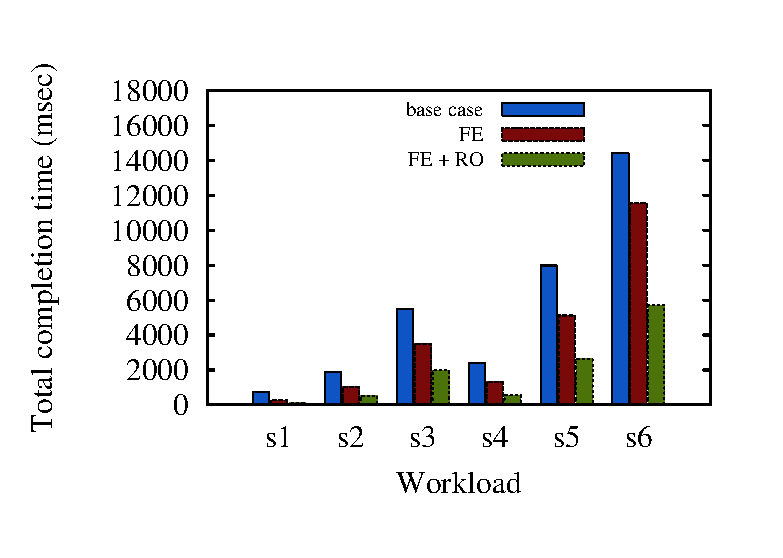
\epsfig{file=./figs/Failover.eps,width=0.35\textwidth}
\vspace{-1em}
\compactcaption{Worst case flow setup time of affected flows in the failover
scenario with \BroadcomOne switches}\label{failoverResults}
\end{figure}

\begin{figure}
\centering
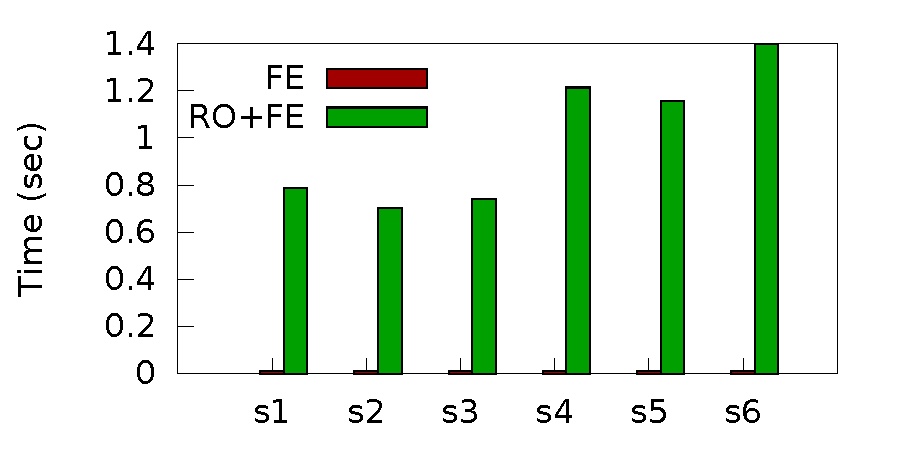
\includegraphics[width=0.3\textwidth]{figs/fe_ro_runtime.pdf}
\botcompactcaption{Running time for FE and RO}\label{runtime}
%\vspace{-0.05in}
\end{figure}

\subsection{Two-level Responsive Traffic Engineering} 
Next, we evaluate the effectiveness of \FE and \RO in the
context of a control application that performs two-level responsive traffic
engineering. This application simultaneously routes two classes of
traffic---high and low priority---over the same network according to
different objectives. For low priority traffic, the objective is to minimize
the overall link utilization of the network due to this traffic; we install
coarse grained (wildcard) rules to route this traffic.  The objective for
high priority traffic is to minimize the overall link latency; we install
fine grained high priority rules to route this traffic. We first route the
low priority traffic, and then route the high priority traffic using the
remaining network capacity. We assume both categories of traffic can be
accommodated without causing any congestion. 

We use the same topology and workloads described in \secref{s:fe_eval}.
However, for high volume workloads (\sD-\sF) the volume of high priority and
low priority traffic between any two overlay nodes is about 17 and 200 flows,
respectively, and for low volume workloads (\sA-\sC) the volume is about 12
and 50 flows, respectively.

%Our experiments above evaluated individual components of Mazu in isolation.
%Next, we consider a network management application where FE and RO (with
%priority handling) both come into play.

%Our application is a two-level responsive traffic engineering scheme
%whose goal is to simultaneously route two categories of traffic --
%high and low priority --
%according to different objectives over the same underlying network.
%This could apply to an ISP that deploys (two classes of) service
%differentiation. The question we address here is how quickly can the network
%establish routes when requests arrive closely in time for both
%categories of traffic. The faster this is, the
%closer the network's ability to meet the SLAs for the corresponding
%classes. This experiment underscores the ability of Mazu to
%help applications that desire fine-grained state control in order
%to meet complex objectives.


%To emulate this, in a somewhat simplistic fashion, we use different objective
%functions to route each category. For routing low priority traffic, the
%objective is to minimize the overall link utilization of the network due to
%this traffic. We install coarse grained (wildcard) rules in the switch to
%route this traffic. The objective for higher priority traffic is to minimize
%the overall link cost, where cost of a link could be  latency. To route the
%high priority traffic we install fine grained high priority rules. These fine
%grained rules could overlap with the coarse grained rules and when they do,
%they have higher rule priority. At first we route the low priority traffic,
%and then on the remaining network capacity we route the high priority
%traffic. For simplicity we assume that both categories of traffic can be
%accommodated without causing any congestion. The rest of the setup is same as
%in \secref{s:fe_eval}. The high and low priority traffic between any pair of
%nodes is proportional to their respective ``popularity'' indices (we assign
%popularity to the nodes at random in the range as shown in
%\tabref{qosTable}). For high volume workloads (s4, s5 and s6) the volume of
%high priority and low priority traffic between any two overlay nodes is about
%17 and 200 flows, respectively, and for low volume workloads (s1, s2 and s3)
%the volume is about 12 and 50 flows, respectively.

A network's ability to meet SLAs for each traffic class depends on how
quickly the network can establish routes when requests for both classes
arrive close in time.
%The faster this occurs, the closer the network's ability to meet the SLAs
%for the corresponding classes. This experiment underscores the ability of
%Mazu to help applications that desire fine-grained state control in order to
%meet complex objectives.
\figsref{qos_Results}{qos_intelResults} show the total completion time using
\BroadcomOne and \Intel switches, respectively, with and without our
techniques. The base case has a significantly high flow set up time when the
number of low priority rules in the table are high: as high as 80s for
\BroadcomOne. This implies that ignoring flow setup latency can cost traffic
engineering dearly in terms of being responsive.  For low volume workloads
(\sA-\sC) the factor of improvement from just \FE is about 2.5X for
\BroadcomOne and 1.8X for \Intel, and with \FE+\RO it's about 5X for
\BroadcomOne and 4X for \Intel. We observe similar speedups for high volume
workloads (\sD-\sF). 





\begin{figure}
% \subfloat[Flow rate = 100/s, concurrent with \flowmod\ and \packetout\ \label{fig:intel_inbound_test1}]
%   {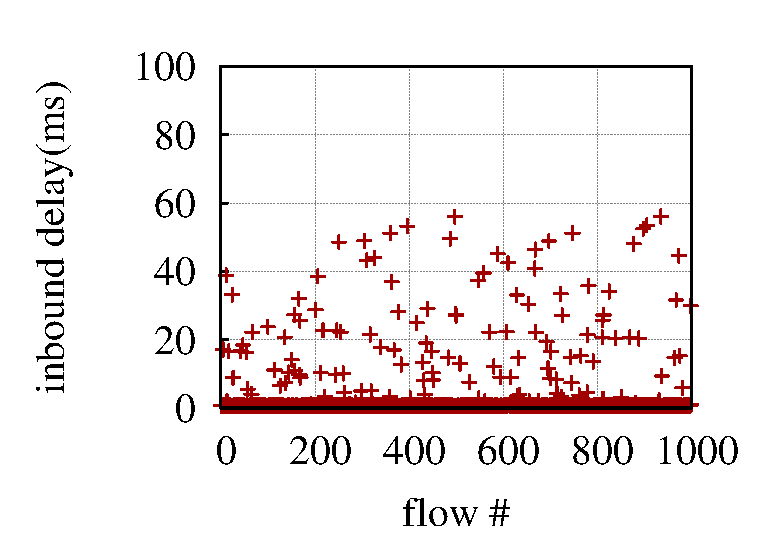
\includegraphics[width=.33\linewidth]{./figs/jan27_intel_inbound_with_pktout_flowmod_rate100.eps}}\hfill
%\subfloat[Flow rate = 200/s\label{fig:hp_inbound_test2}]
%  {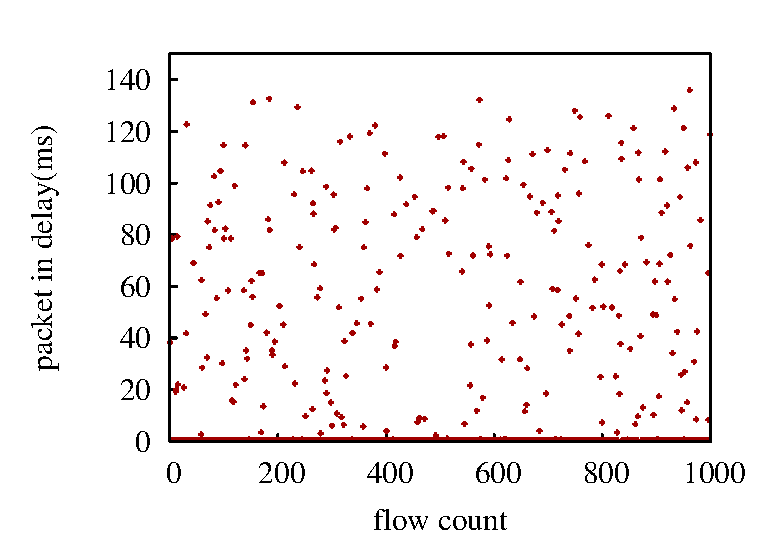
\includegraphics[width=.28\linewidth]{./figs/hp_inbound_delay_200.eps}}\hfill
\subfloat[Latency on \BroadcomOne switch \label{qos_Results} ]
  {\includegraphics[width=.5\linewidth]{./figs/qos.eps}}
\subfloat[Latency on \Intel switch \label{qos_intelResults} ]
  {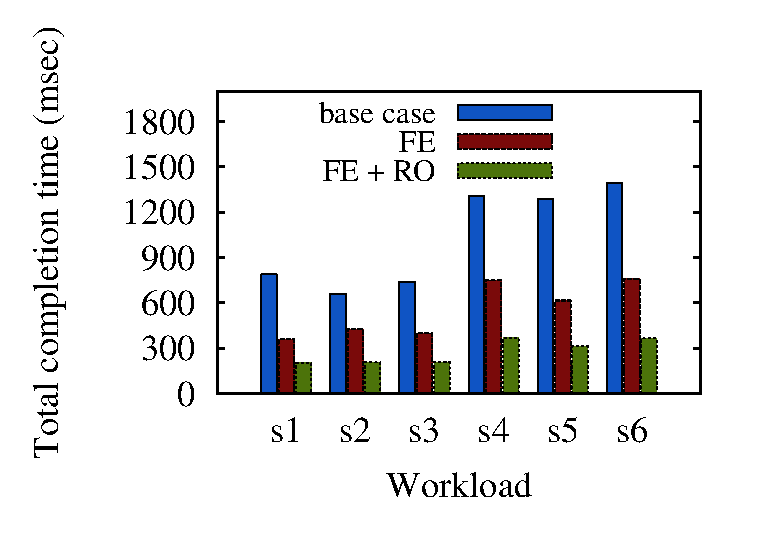
\includegraphics[width=.5\linewidth]{./figs/qos_intel.eps}}
\compactcaption{Worst case flow set up time in the two level traffic
    engineering scenario} 
%with base case, FE and FE+RO techniques in a full mesh topology with 25 nodes}
\label{qosResults}
\end{figure}

\subsection{MicroTE}
%Rule Offload in Isolation} 
%Lastly, we study the benefits of RO in isolation.

%\minisection{ClassBench} 
%While the above scenarios did leverage rule offload, the rules inserted had a
%flat priority structure and did not have dependencies. In what follows, we
%study how well rule offload works when these simplifying criteria may not
%apply.  
% We leverage ClassBench~\cite{classbench} to generate a variety of rule
% sets representative of real world access control. Since
% dependent rule sets, in most cases, hinder rule offloading to the next hop
% switches, we believe that the ACL rule sets generated by ClassBench---which
% have many dependen\-cies---present a near worst case scenario for our RO scheme.

% \begin{figure}[!tb]
% \centering
% %%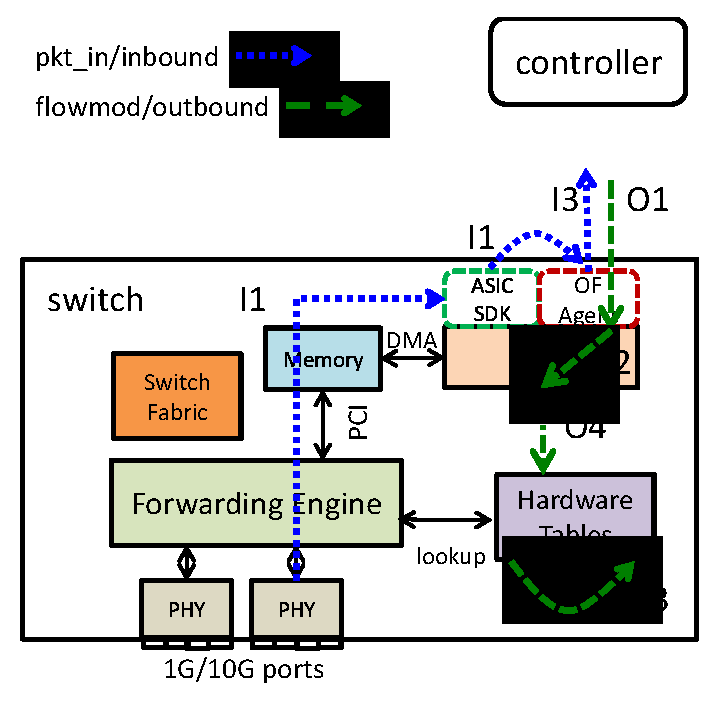
\epsfig{file=./figs/openflow_switch_illustrate.eps,width=0.35\textwidth} %%changed
% 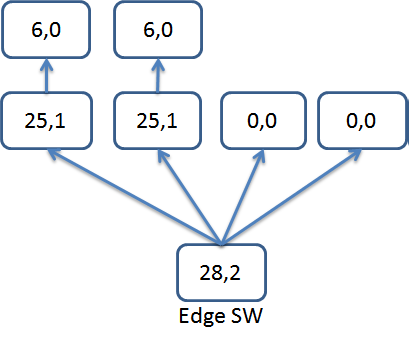
\includegraphics[width=2.5in]{figs/ruleoffload_cb.png}
% \caption{rule offloading from an edge switch with 90 rules to its
% next hops. The numbers a,b (e.g. 28,2) denotes the number of rooted
% rules and default rules
% respectively. }\label{experiment_setup} \end{figure} 


% We consider the following simple setup: we use a three-level FatTree
% topology~\cite{fattree-sigcomm08} with degree 8, containing 128 servers
% connected by 32 edge, 32 aggregate, and 16 core switches.  We use ClassBench
% to generate 90 rules for each edge switch. Each rule is assigned a different
% priority and a tunnel tag to indicate its tunnel or path. 
% Without RO, assuming one-shot updates, the installation time will be
% the maximum at any edge switch when inserting 90 rules. With RO, we assume a
% core switch cannot accommodate more than 60 rules in total from {\em all} of
% its immediate upstream neighbors.

% We experimented with a variety of rule sets. On average, the speedup
% from using RO relative to not using it is 2.1x for \BroadcomOne switches and
% 1.4x for \Intel switches. This speedup is made possible by RO ``spreading''
% rules to downstream switches, enabling parallel execution of updates. 

% To show how rule offload works, we present the distribution of the
% offloaded and default rules across the network in Figure
% ~\ref{classbenchResults}. The switch IDs from 0-31 denote the edge
% switches, each having 90 rules to be inserted, 32-63 denote
% aggregate switches and 64-89 denote core switchs. Figure shows the
% overall rule distribution of accross the network as a result of rule
% offload.   

% We apply the rule offloading algorithm on each of the rule sets to
% generate the partitions to offload the rules. Once the partitions
% are generated for the switches each containing rules of differing
% priorities to be installed on that switch, we calculate the total
% insertion latencies incurred in the best case scenario (increasing
% order for Intel and decreasing order for broadcom) to insert those
% rules . We repeat this experiment for  different rule set generated
% using Class Bench and then calculate the average completion
% time. Since, all the offloaded rules and the remaining rules at the
% edge switches can be inserted in parallel, this technique proves to
% be very effective in reducing the overall rule insertion completion
% time. In our simulations, we observe that the speed up in completion
% time for topology with Broadcom and  Intel switches to be 2.1 and
% 1.4 respectively. 

% \begin{figure}[!tb]
% \centering
% 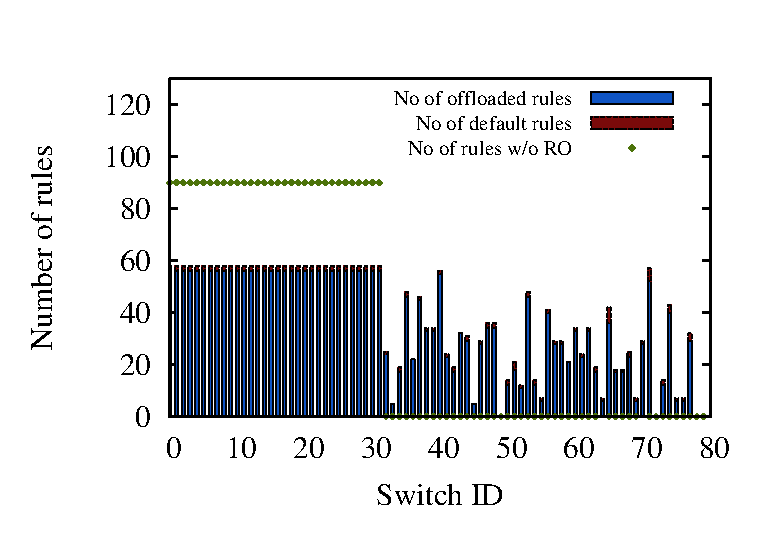
\epsfig{file=./figs/ClassBench_RuleDist1.eps,width=0.4\textwidth}
% \caption{ Rule offloading using ClassBench rules on Fat Tree topology (k=8). Distribution of rules across the network }\label{classbenchResults}
% \end{figure}

% \minisection{MicroTE} We now consider an important scenario discussed in
% \secref{sec-motivation}: fine-grained intra-DC traffic engineering using
% MicroTE~\cite{microte}. 
MicroTE~\cite{microte} leverages the partial and short term
predictability of a data center traffic matrix to perform traffic engineering
at small time-scales. As noted in \secref{s:floweng}, \FE does not apply to
MicroTE since routes span a single tunnel and route changes all happen at a
single switch. Thus, MicroTE can only benefit from \RO, the extent of which we
now study.




% We examine the performance of our flow offloading module under varying levels of workloads. We use MicroTE, a traffic 
% engineering application, to evaluate the performance for an independent rule set, and class bench to generate real world rule sets with dependent 
% rules.


% {\bf Rule offload without dependencies}

% We use MircoTE to examine the effectiveness of rule offload on a 
% rule set without dependencies.
We consider the following simple data center topology: we use a three-level FatTree topology~\cite{fattree-sigcomm08} with degree 8, containing 128 servers connected by 32 edge, 32 aggregate, and 16 core switches.
%We use the same data center topology as discussed earlier in this section. 
We
assume that the traffic rate between a pair of servers is derived from a
Zipfian distribution. \figref{microteResults} shows the rule installation
completion time. We see that \RO provides a 2X improvement (400ms to 200ms)
assuming the \BroadcomOne switch. Given the time-scales of predictability
considered, this can help MicroTE leverage traffic predictability longer,
thereby achieving more optimal routing. The improvement with \Intel is 1.6X
(80ms to 48ms).

%  MircoTE with flow offloading has 40\% improvement with intel's switch model and 50\% with broadcom's witch model in overall competition time.

\begin{figure}[!tb]
\centering
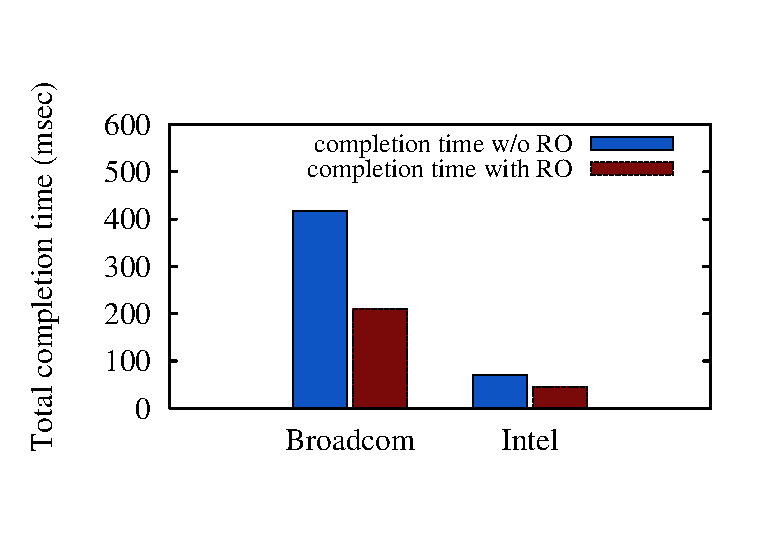
\epsfig{file=./figs/MicroTE_Compl.eps,width=0.65\columnwidth}
\vspace{-1em}
\compactcaption{Flow setup time of MicroTE with and without \RO in a Fat Tree (k=8) topology}\label{microteResults}
\end{figure}

%In summary, all of Mazu's mechanisms are crucial to ensuring that route
%setup is sufficiently fast.

%%  for management applications that desire
%% fine-grained control to achieve complex objectives.
